% Read This:
% Notation:
% ??? = unsure about something, some flaw in Text, something is missing
% !!! = there is still work to do here




\documentclass[12pt]{article}

%\usepackage{biblatex}

\usepackage{graphicx}         % fuer das Einbinden von Grafiken
\usepackage{caption}       
\usepackage{comment}  
\usepackage{float}
\usepackage{subcaption}
\usepackage{amsmath}					%Um Formeln einzugeben
\usepackage{amssymb}					%Sonderzeichen und Symbole	
\usepackage{hyperref}
\usepackage{listings}
\usepackage[utf8]{inputenc}





\RequirePackage[backend=biber,
    sorting=none, % http://tex.stackexchange.com/a/51439
    maxcitenames=2]{biblatex} %% biber with biblatex
\DeclareFieldFormat{apacase}{#1} % disable case altering
\newrobustcmd{\citeright}[1]{\begin{flushright}-- \citeauthor{#1}, \citeyear{#1}\end{flushright}} % like \cite{} but with a dash and aligned to the right
\addbibresource{sources.bib}

\usepackage{siunitx}


% Title Page
\title{AML Final Project: Creating an Image Input Calculator} %Ullrich Köthe
\author{Timothy Jay Herbst, Fenja Kollasch, Duc Anh Phi}

\begin{document}
\maketitle

\begin{abstract}
	This paper deals with the development of a calculator, which can infer, from an image of an equation, its solution.
	To do this, the image will, after going through some preprocessing, be segmented into the separate symbols that make up the equation.
	These symbols will then be ordered and classified, which allows solving of the equation.
	While similar projects exist, this project goes into detail, how this can be done.
	And, being open source, demonstrates, how such a problem may be tackled and gives a sophisticated basis for many other projects on a variety of topics.
	
	
	
\end{abstract}
\newpage

\tableofcontents

\newpage
\section{Motivation}

Computers are superior to humans in many everyday disciplines.
A Calculator, for instance, uses less time to calculate the solution of most simple mathematical problems than it does for the user to enter the equation.
This has inspired us to search for a solution to this flaw in a common household item.
If we want to improve upon calculators, we will not have to increase the speed at which computers calculate.
Instead the focus should lie on improving the efficiency of entering an equation into the calculator.\\
We decided to make a calculator able to find the solution of equations, when given an image of the equation.
In the following paper we will explain, how such a calculator can be designed.\\
We hope that this serves as an inspiration to solve similar issues, and that the code provided proves useful.

\section{Introduction}
The creation of an automatic image input calculator for handwritten formula mainly combines two common computer-scientific problems. 

For once, several operations from visual computing need to be applied to the image. The application has to segment the input image into one segment per character. It is important that the ordering of these symbols is preserved during this step. Otherwise, it would not be possible to reconstruct the original formula.

The second issue our program has to address, is the recognition of each segmented character. To do so, we can apply methods from machine learning. Luckily, the recognition of handwritten symbols is a well-known problem that has been approached by various researchers before. LeCun et al \cite{lecun1998} for instance discussed different methods to recognized handwritten digits in 1998. With this work, they made a huge contribution by providing this MNIST database of handwritten digits \cite{mnist} that is used for many toy examples in machine learning. In fact, the task that is solved around the MNIST dataset does not differ very much from our own classification task. Symbols that can appear in a calculator input will mainly be digits from 0 to 9. Additionally, mathematical operators, brackets, latin symbols and greek symbols could be found in a mathematical formula. For this work however, we will focus on recognizing only digits and simple mathematical operators like plus, minus, multiplication-, and division symbols, as well as brackets.

After these two major steps are complete, there is only one task left. Reconstructing the formula with the recognized symbols, and aligning them in the order in which they appeared on the input image to finally evaluate the term and present the result.

	

\section{Preprocessing}
	Our program receives at first a simple unaltered image.
	From this image it is difficult to detect significant features, such as the symbols that make up the equation.
	Therefore, it is necessary to do some preprocessing, before further steps make sense.\\
	We are facing several issues in this.
	Some improvements we could make include:\\
	\begin{itemize}
		% !!!
		\item Correction for different Quality of Camera, Lighting, etc.:
		The incoming images vary to a great extent due to changes of lighting and may come from different cameras.
		Correcting for this, is not a simple task.
		A future improvement of this project would improve greatly by having an adaptive preprocessing step.
		% !!!
		\item Simplification of the input dimensions: Explicitly we want our image to be a black-white image, with the only two colours being black (0) and white (255).
		\item Connectedness of the symbols: For later steps it is useful to not segment any symbols. In the same manner we do not wish for two different symbols to be connected.
		\item Removal of Noise: Often the background (e.g. paper or whiteboard) is not uniform and this can create spots on the image. (The human eye is very good at filtering these out.)
		\item Background Contour removal: Often times when taking an image of a contour there will be other objects in the image (e.g. pencils, the border of the paper, etc.).
	\end{itemize}
	%!!! ??? Add more
	We correct for (most of) these issues in two separate steps:\\
	At first we use a few select image processing steps to deal with most of the issues.\\
	In a second step we remove the contours that can be attributed to background objects.

	\subsection{Simple Preprocessing}%??? !!! Add stepwise Images, after Preprocessing is complete
		The image our programm receives as input is likely not easily analysed.
		We therefore manipulate the image with a few select operations, before continuing with our algorithm.
		It should be noted here, that there is a great variety of different algorithms that work well.
		The algorithm we will be presenting here is the one, we found to be the most usefull for our purpose.\\
		It operates in five steps:
		\begin{itemize}
			\item Grayscaling: At first we grayscale our image. Here we reduce the BGR (blue, green, red) image into an image with a single dimension per pixel. This is usefull, because this simplifies our image and allows us to more easily analyse the image.
			\item Gaussian Blur: Here we apply a gaussian blur kernel on the image to smooth it out. This reduces the noise.
			\item Morphological Opening: We apply a filter that removes a specific type of noise: Small dots. This is done by applying an erosion followed by a dilation filter. %??? is this the right filter
			\item Adaptive Threshold: We add a filter that applies a threshold. Any pixel below this threshold gets set to 0 any pixel above it gets set to 255. %??? check
			This threshold differentiates the symbols from the background.
			We will later explain in more precision how this filter works. %??? !!! Do it
			\item Dilation: After the previous steps it is possible that some of the symbols have deteriorated into several parts. %??? Errosion is Dilation correct?
			(Because our image is inverted, the code uses an erosion function.) %??? fix
			Therefore, it is useful at this point to thicken the contours.
		\end{itemize}
		\begin{lstlisting}
	def preprocess(self, img):
		preprocessed = self.convert_gray(img)
		preprocessed = self.gaussian_blur(preprocessed)
		preprocessed = self.morph_open(preprocessed)
		preprocessed = self.binarize(preprocessed)
		preprocessed = self.erode(preprocessed)
		return preprocessed
		\end{lstlisting}
			
	
	\subsection{Border Removal}%??? !!! Add before vs after Images, after Preprocessing is complete
		After the steps above, we determine a fairly good image.
		However, very often the shape of background objects register as contours.
		Our mission in the following section is to be able to remove the contours of background objects.
		For this we make use of a simple observation: Symbols tend to be separate from other contours, while background contours tend to be flaky and can be roughly traced to the border of an image, see fig .%???
		Using this knowledge we can create a mask, which removes the background contours.\\
		We determine the mask in the following steps:
		\begin{itemize}
			\item Simple Preprocessing: At first we need to simplify the image. We use a similar algorithm as used in the section "Simple Preprocessing" for this.
			\item Adding a Border: For the next step we add a black border to the image. Our aim is to remove all contours which connect with this border.
			\item Strong Dilation: We now repeatedly dilate the image. Our goal here is to connect all contours which are close to each other.
			Unfortunately this makes our contours unreadable.
			This is not a problem since in this step we simply want to determine the contours we want to keep.
			\item Floodfill Border: We then floodfill the border.
			This removes any contour which connects to the border. 
			\item Remove Border: Since we changed the image size by adding a border, we now have to remove it.
		\end{itemize}
		In this manner we determine the mask.
		Our resulting image is determined, by having all pixels white, except those, that are black both in the mask and in the simple preprocessing.
		This removes background contours, without making our image unreadable.
	
	\subsection{Adaptive Threshold} %??? !!! Add before vs after Images, after Preprocessing is complete
		A problem we face with the images, is that we do not know if a pixel is part of the writing or not.
		The "Adaptive Threshold" function \cite{adaThresh}, found in the openCV library is very useful in this case. %???
		This function operates like most threshold functions, in that it compares a pixel to a threshold $T$.
		If the pixel is found to have a value higher than the threshold $T$, we set it to 255.
		Otherwise the pixel is set to a value of 0 \cite{cvAdaThresh}
%		\begin{align}
%			newImg(x,y)=
%			\left
%			\begin{cases}
%			255  \hspace{1cm}&\mathrm{if} \hspace{0.5cm} img(x,y)>T \\
%			0  &\mathrm{else}
%			\end{cases}
%			\right.
%		\end{align}
		This way it is possible, to easily "classify" a pixel as writing (0) or not (255).\\
		What makes this function work so well, is that for every pixel the threshold $T(x,y)$ is calculated separately.
		While there are several different ways, how we can calculate this, it was found to work best for our problem, by a simple process [2]:\\
		The threshold $T(x,y)$ is set to the gaussian weighted sum of every pixel within a window with side length 11 (extends 5=(11-1)/2 pixels out from (x,y)):
		\begin{align}
			T(x,y)=&\sum_{\Delta x=-5}^{5}\sum_{\Delta y=-5}^{5} -2 + G_{(\Delta x,\Delta y)} \cdot img(x+\Delta x,y+\Delta y)\\
			\mathrm{with}& \hspace{1cm} G_{(\Delta x,\Delta y)} = \alpha \cdot \mathrm{exp}(-(\Delta x ^2 +\Delta y^2)/(2*\sigma)^2)\\ %??? check
			&\mathrm{with} \hspace{1cm}\alpha = 1/\Big(\sum G_{(\Delta x,\Delta y)}\Big)\\
			&\mathrm{with} \hspace{1cm}\sigma = 0.3 \cdot ((11-1)/2-1) + 0.8 = 2
		\end{align}
		Here $\alpha$ is the normalisation factor and $\sigma$ is the recommended standard deviation for a box size of 11.
	
%??? maybe add this	\subsection{Small Contour Filter Mask}
		
	
	
\section{Segmentation}

\section{Line Assigning and Ordering}
	After finding the Contours we now face the problem, of bringing them into an order, where they then can be classified and calculated.
	We order them before classifying them, because this allows us to remove certain contours, based on criteria, we will go into later.
	This saves the program from having to classify contours caused by noise.
	Thereby our program becomes more efficient.
	It also becomes possible to classify some symbols, based on their size and position.
	Thereby, we can reduce the amount of classes we need to identify with the classifier. \\
	For the Line Assigning we have developed several algorithms, of which we will be discussing the most interesting, the ones able to tackle a particular problem and the most efficient ones.
	
	\subsection{Problems with Determining Line Order}
	
	
	\subsection{Determining the Direction of Writing}
	When writing an equation, most people tend to write roughly along an "invisible line".
	Therefore, when taking an image of said equation, we can expect it to adhere roughly to the line.
	We can use this to determine the order of the symbols.\\
	There are however, two issues with this:\\
	Firstly, unlike a computer a human will not precisely write their symbols in a line.
	Oftentimes a symbol will be significantly above or below said line.
	It gets even worse, if we take a look at exponents, division bars and similar.\\
	Secondly, the "invisible line" may not be along the horizontal of an image.
	This may be because of sloppiness of the writer, or because the image was taken at an angle.\\
	Because of this, it is very useful to be able to determine the direction of such an "invisible line".
	In the following we will be discussing a method how to determine this line.
	It should be noted at this point however, that in most images we took this "invisible line" deviates by less than $10$.
	All of the following algorithms are capable of dealing with such small deviations.\\
	
	
	
	%\subsection{A Naive Approach}
	%This section aims not to introduce a particular algorithm, but to illustrate some of the problems such an algorithm must face.
	
	%A naive approach to assigning lines, may be to assume two symbols are within the same line, if they are close to each other.\\
	%This could be implemented, by determining a radius of acceptance $R$.
	
	\subsection{Assigning Lines to Proposed Line Positions}
	Our aim is to accurately order the contours into lines.
	A possible method for doing this is by proposing the position of lines.
	Then we check for each proposed line, whether or not a given contour is a good fit (if it is within a certain radius of the line).\\
	For this procedure we at first have to find a rough estimate of the diameter of a line.
	This can be done in a variety of different ways.
	The best method we found at first determines the extension (radius of minimal enclosing circle) of every single found contour.
	Of these, the biggest radius that isn't part of a fraction is then chosen to be the presumed line radius.\\
	To find the ideal line position, we propose a great variety of possible lines.
	In practice we choose a line every $0.4 \cdot \mathrm{line radius}$.
	For every one of these lines, the appropriate contours are assigned.
	Because we choose a lot of different lines, it is very likely that contours are present in multiple lines.
	We can find the best lines, by removing all lines, that have a neighbouring lines, which contain more symbols.
	The longest lines correspond to the written lines.\\
	Afterwards, all lines with less than 3 symbols in them are removed.
	This can be done with confidence, because even the smallest equation (e.g. "1+1") has at least 3 symbols.\\
	
	While there are some obvious flaws with this method, it works surprisingly and consistently well.
	It performs especially well, when equations are written along lines with large spaces between symbols.
	Compared to other methods it can maintain the position of a line and doesn't wander into other lines.\\
	It does however, have difficulty if there are hazy patches in an image, which cause a large amount of wrong contours close to each other.
	The algorithm will always attempt to place a line around these contours.\\
	Another issue is caused, if the lines are written too close and there is a large contour.
	If this is the case, then the line might be placed in between both lines and use contours from both lines.
	%!!! ??? Add more issues
	%!!! ??? Add images
	
\section{Symbol Classification}
After the preprocessing routine is complete, each handwritten character is extracted from the original image. The correct order in which the characters will appear in the term is also known. Now, the remaining challenge is to recognize the characters and assign the correct labels such that an evaluation of the written term can take place.
	
	Therefore, we need to solve a typical classification problem. It is similar to the classification of the \textit{MNIST} image data set including 60000 images of handwritten digits. Additional to the digits from 0 to 9, our classifier also needs to recognize the symbols \textit{+}, \textit{(}, and \textit{)}, as well as the letters \textit{x} and \textit{y}. All kinds of dashes like the ones used in an equal sign or a minus symbol will not be recognized by machine learning techniques but will be handled by manual classification.
	
	To classify the image, we use a deep convolutional neural network (CNN). The network will be trained in beforehand. During the use of our main application, the segmented and preprocessed images of the characters are going though the forward pass of the trained model. The labels that were assigned during this process are furthermore send to the symbolic math solver to evaluate the result of the term. 
	
	The framework containing most of the machine learning functions we are using, is \texttt{pytorch}. We decided to use \texttt{pytorch} because we familiarized ourselves with this library during the exercises of this class. Furthermore, \texttt{pytorch} offers complete models suitable for classification.
		
	Dash- or dotlike symbols however are extremely hard to recognize automatically, since they cause major overfitting within the network. A highly accurate classifier is crucial for our program to work. For this reason, we perform a manual classification of difficult symbols and leave the automatic classification for symbols with distinctive features.
	
	\subsection{Training data}
		To create a well trained model, a sufficient amount of training data is crucial. For the training routine, we decided to use two public data sets of handwritten symbols. Additionally, we created some training images ourselves that are created the same way as the input of the future classifier in our system. All of these images merge into a combined data set which will be finally used to train the character classificator.
		
		We created our own instance of the \texttt{Dataset} class provided by \texttt{pytorch} to capsule the data. It is crucial that the training data resembles the images created by our application as well as possible. Therefore, we apply an individual preprocessing routine to each dataset. Usually, this contains all steps made during the preprocessing of the segmented images. Additionally, the \texttt{numpy} arrays describing the images are transformed into \texttt{PIL} images. By doing so, we are able to apply some transformations to the images which are offered by \texttt{pytorch} to create some data augmentation. Furthermore, we resized them to 32*32 pixels. All images are converted to 1-channel grayscale and inverted to have a black background and white content. Finally, the images are transformed to \texttt{pytorch} Tensors to make them suitable for the neural network. 
		
		\subsubsection{MNIST}
			As a basic training routine, we used the already mentioned MNIST database of handwritten digits. \texttt{pytorch} offers the MNIST data directly. However, the format in which the images are provided by \texttt{pytorch} is not suitable with the preprocessing routine that makes mainly use of the \texttt{opencv} functions. Therefore, we gather the data not from \texttt{tensorflow}. The images are converted to \texttt{numpy} arrays. Afterwards all necessary operations get applied and the preprocessed images will be saved. 
			
			To finally include the preprocessed images in the combined dataset, we provide a function to load the images again, convert them into \texttt{PIL} images, apply the necessary transformations and make them into tensors.
			
		\subsubsection{HASY}
			Mathematical symbols need to get recognized as well. To include these symbols in our training process we extended our training data with a subset of the HASYv2\cite{hasy} dataset. This dataset contains 168233 images in total which can be labeled with one of 369 classes including all numbers and latin letters. 
			
			Not all symbols in this dataset are relevant for our classifier. Therefore, we filter the images according to their labels and thus simply include the ones that are necessary for our training procedure. Our first approach was to take only the digits and plus symbols from this dataset. Unfortunately, many of the digit images were cropped or of poor quality. In the end, we decided to take only the plus symbols from the dataset what leaves us with roughly 100 images after the filtering. Since MNIST contains 60000 images of digits, we have a critical overflow of digit characters in comparison to the plus symbols. To reduce this gap, we make use of data augmentation and apply a number of transformation to all non-digit characters. By rotating, flipping and combinations of rotation and flipping we generate four extra images per non-digit symbol and remain now with 405 training images.
			
		\subsubsection{Custom training images}
		Furthermore, we generated some training images ourselves by writing down symbols and capture them the same way in which our application will capture the mathematical formula during usage.
		
	\subsection{Training}
		A \textit{Jupyter notebook} is provided for the complete training routine. First of all, the combined dataset is loaded for test and training data. This dataset includes images from MNIST, HASY, and our own images as well. Since the class that holds our dataset inherits from \texttt{pytorch}'s class \texttt{Dataset}, we are allowed to use a \texttt{DataLoader} for training. The \texttt{DataLoader} class makes it possible to iterate in a comfortable way over the minibatched dataset. We use minibatches of the size of 16 samples per batch. The training is running over 10 epochs.
		
		Stochastic optimization is done by using an \textit{ADAM}\cite{adam} optimizer. Since it is claimed to work best on classification issues with multiple classes, we use cross entropy loss as a loss function.
		
		We decided to leave 11 different symbols to the automatical classification: The digits from 0 to 9,  and \textit{+}. Therefore, the classification problem we are trying to solve is very close to MNIST what makes the chances high to achieve a good accuracy. Other operators will be classified in an earlier step in a manual way. Thus, our classifier needs to map the images to one of 15 labels.
				
		\subsubsection{Neural network}
		
		\begin{figure}[h!]
			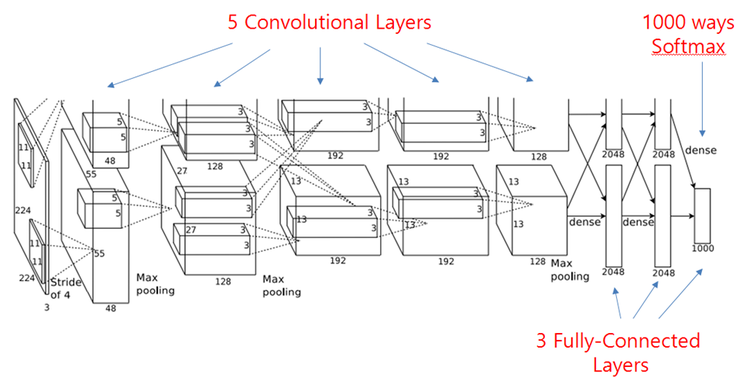
\includegraphics[width=\textwidth]{alexnet2.png}
			\caption{The AlexNet architecture}
			\label{fig:architecture}
		\end{figure}
		The network architecture we decided on is \textit{AlexNet}\cite{alexnet}. Thus, the network contains five convolutional and three fully connected layers. The convolutional layers are followed by max-pooling layers while some dropout layers are placed before the linear layers (see figures \ref{fig:architecture}). An implementation of \textit{AlexNet} is provided by \texttt{pytorch}. Since the model is suited for images with three color channels we modified the first layer to accept images with only one channel. On the next page, a summary of the network is displayed. It shows, which layers the network contains and how these layers look like.
		\newpage
			\begin{lstlisting}
AlexNet(
  (features): Sequential(
    (0): Conv2d(1, 64, kernel_size=(7, 7), stride=(2, 2),
     padding=(3, 3), bias=False)
    (1): ReLU(inplace)
    (2): MaxPool2d(kernel_size=3, stride=2, padding=0,
     dilation=1, ceil_mode=False)
    (3): Conv2d(64, 192, kernel_size=(5, 5), stride=(1, 1),
     padding=(2, 2))
    (4): ReLU(inplace)
    (5): MaxPool2d(kernel_size=3, stride=2, padding=0,
     dilation=1, ceil_mode=False)
    (6): Conv2d(192, 384, kernel_size=(3, 3), stride=(1, 1),
     padding=(1, 1))
    (7): ReLU(inplace)
    (8): Conv2d(384, 256, kernel_size=(3, 3), stride=(1, 1),
     padding=(1, 1))
    (9): ReLU(inplace)
    (10): Conv2d(256, 256, kernel_size=(3, 3), stride=(1, 1),
     padding=(1, 1))
    (11): ReLU(inplace)
    (12): MaxPool2d(kernel_size=3, stride=2, padding=0,
     dilation=1, ceil_mode=False)
  )
  (avgpool): AdaptiveAvgPool2d(output_size=(6, 6))
  (classifier): Sequential(
    (0): Dropout(p=0.5)
    (1): Linear(in_features=9216, out_features=4096, bias=True)
    (2): ReLU(inplace)
    (3): Dropout(p=0.5)
    (4): Linear(in_features=4096, out_features=4096, bias=True)
    (5): ReLU(inplace)
    (6): Linear(in_features=4096, out_features=15, bias=True)
  )
)
		\end{lstlisting}
		\newpage
		
	\subsubsection{Hyperparameter training}
	\texttt{pytorch} allows to set the training hyper parameters. The ones that are relevant in our routine are the learning rate, the beta values for the \textit{ADAM} optimizer, and the weight decay. To find the optimal values for these parameters, we created a second notebook in which we trained under the same conditions for one epoch with different hyperparameter values and compared the achieved accuracies. Table \ref{tab:hyperparams} shows which values we tried out for each parameter. The best results were achieved with a learning rate of 0.001, a beta tuple of (0.95, 0.95), and a weight decay of 0.
	\begin{table}[h!]
		\begin{tabular}{c|c}
			\textbf{Parameter} & \textbf{Values} \\
			\hline
			Learning rate & 0.01, 0.001, 0.0001 \\
			Beta 1 & 0.8, 0.85, 0.9, 0.95 \\
			Beta 2 & 0.9, 0.925, 0.95, 0.99 \\
			Weight decay & 0, 0.01, 0.001, 0.0001
		\end{tabular}
		\caption{The values we evaluated for the different hyperparameters}
		\label{tab:hyperparams}
	\end{table}
	
	\subsection{Automatic Classification}
	After the training is complete, we save the model to a \textit{.ckpt} file. The actual classifier that will be used in our program will be an instance of the class \texttt{MathSymbolClassifier}. This class simply contains an \textit{AlexNet} instance in which we load the information from the trained model. To predict what each of our segmented images shows, the class provides a function \texttt{classify}. The function takes a \texttt{numpy} array with images as an input, creates a tensor out of this array and leads the data through the network. Afterwards the predicted label is returned as a string and can be furtherly processed by the symbolic math solver.
	
	\subsection{Manual Classification}
	Before the extracted symbols are given as an input for the automatic classifier, we check manually if they picture a symbol that our classifier can not recognize. This applies for opening and closing brackets, minus symbols, equal signs, commas, and multiplication dots.

\section{Calculations}

\section{Discussion}
	In this section, we will discuss the progression of this project regarding the result.
	\subsection{Classification problems}
	A major issue appearing during development was the fact that the usability of our application highly depends on the accuracy of the classifier. Our initial ambition was to recognize various more symbols automatically. Unfortunately, we were not able to gather enough training data and therefore we could not create models with the desired accuracy. Any classifier that recognizes less than 95\% causes major leaks in the overall performance of our program and makes it unusable. Furthermore, it took a long time to create well-trained models what made the training procedure tedious and decelerated our progress.

\section{Conclusion}

\newpage
\printbibliography[heading=bibintoc, title={Sources}]
%??? !!! Create bibliography
%	[1] $https://www.tutorialspoint.com/opencv/opencv_adaptive_threshold.htm$ \\
%	[2] $https://docs.opencv.org/2.4/modules/imgproc/doc/miscellaneous_transformations.html?highlight=adaptivethreshold$

\end{document}          
